\scanpage{51}
% archive sheet number: 50
$A$ anneau \unsure{régulier}, de dim finie, \deleted{\unsure{biéquidimensionnel}}

\[
\begin{aligned}
\deleted{D(A)=\coprod_p\underbrace{D_p(A)}_{I_p}}\\
\deleted{DD(A)=\prod_{\unsure{p|qp}}\operatorname{Hom}(I_p,}
\end{aligned}
\]

\[
D(M)=\operatorname{Hom}(M,K_*)=\coprod_p
\underbrace{\operatorname{Hom}(M,\deleted{\unsure{I_p|K_p}}K_p)}_{p\text{-primaire}\quad D_p(M)}
\]
\[
DD(M)=\prod_p\operatorname{Hom}(\deleted{\unsure{D_q(M)|D_p(M)}}D_p(M),K)
\]

\[
D_p(M)=\varinjlim_i U_i
\qquad\text{les $U_i$ sont de longueur finie sur $A_p$.}
\]
\[
\operatorname{Hom}(D_p(M),K)=\varprojlim_i\underbrace{\operatorname{Hom}(U_i,K)}
\]
\[
\operatorname{Hom}\unsure{(}U_i,K_*)=\coprod_q\operatorname{Hom}(U_i,K_q)
\]
\[
\operatorname{Hom}(U_i,K_q)=\varinjlim_j\operatorname{Hom}\unsure{(}U_i,
\underbrace{K_{q,j}}_{\substack{V_j\text{ de longueur}\\\text{finie sur}\\A_q}})
\]

\figure{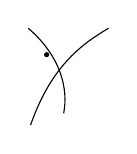
\begin{tikzpicture}[scale=.6]
\draw (-.6,1.2)..controls (.1,.6) and (.25,-.1)..(.15,-.6);
\draw (-.55,-.85)..controls (-.1,.45) and (.6,.9)..(1.1,1.2);
\fill (-.21,.64) circle (.055);
\end{tikzpicture}}

Or $\operatorname{Hom}\unsure{(}U_i,V_j)=0$ si $\unsure{q\not\supset p|q\ne p}$;

donc on aura $\operatorname{Hom}(U_i,K_q)=0$ si $q\not\supset p$,

d'où
\[
\operatorname{Hom}\unsure{(}U_i,K_*)=\coprod_{\underline{\underline q}\supset p}\operatorname{Hom}(U_i,K_q)
\]
\[
\begin{aligned}
DD(M)&=\prod_p\operatorname{Hom}(D_p(M),\coprod_{\underline{\underline q}\supset p}K_q)\\
&=\prod_p\prod_{\underline{\underline q}\deleted{\unsure{\supset}}\unsure{\supset}p}^{\mathrm{local}}\operatorname{Hom}(D_p(M),K_q)
\end{aligned}
\]
